\onecolumn
\chapter{Anhang}
\begin{table}[h!]
\centering
\begin{tabular}{c|c||c|c}
\hline
T [°C] & $p_D$ [Torr] & T [°C] & $p_D$ [Torr] \\
\hline
10 & 9,20  & 31 & 33,70 \\
11 & 9,84  & 32 & 35,67 \\
12 & 10,51 & 33 & 37,73 \\
13 & 11,23 & 34 & 39,90 \\
14 & 11,98 & 35 & 42,18 \\
15 & 12,78 & 36 & 44,57 \\
16 & 13,63 & 37 & 47,08 \\
17 & 14,53 & 38 & 49,70 \\
18 & 15,47 & 39 & 52,46 \\
19 & 16,47 & 40 & 55,34 \\
20 & 17,53 & 41 & 58,36 \\
21 & 18,65 & 42 & 61,52 \\
22 & 19,82 & 43 & 64,82 \\
23 & 21,07 & 44 & 68,28 \\
24 & 22,38 & 45 & 71,90 \\
25 & 23,76 & 46 & 75,67 \\
26 & 25,21 & 47 & 79,63 \\
27 & 26,74 & 48 & 83,75 \\
28 & 28,35 & 49 & 88,09 \\
29 & 30,04 & 50 & 92,60 \\
30 & 31,82 &    &       \\
\hline
\end{tabular}
\caption{Sättigungsdampfdruck von Wasser}
\end{table}

\newpage

\begin{figure}
    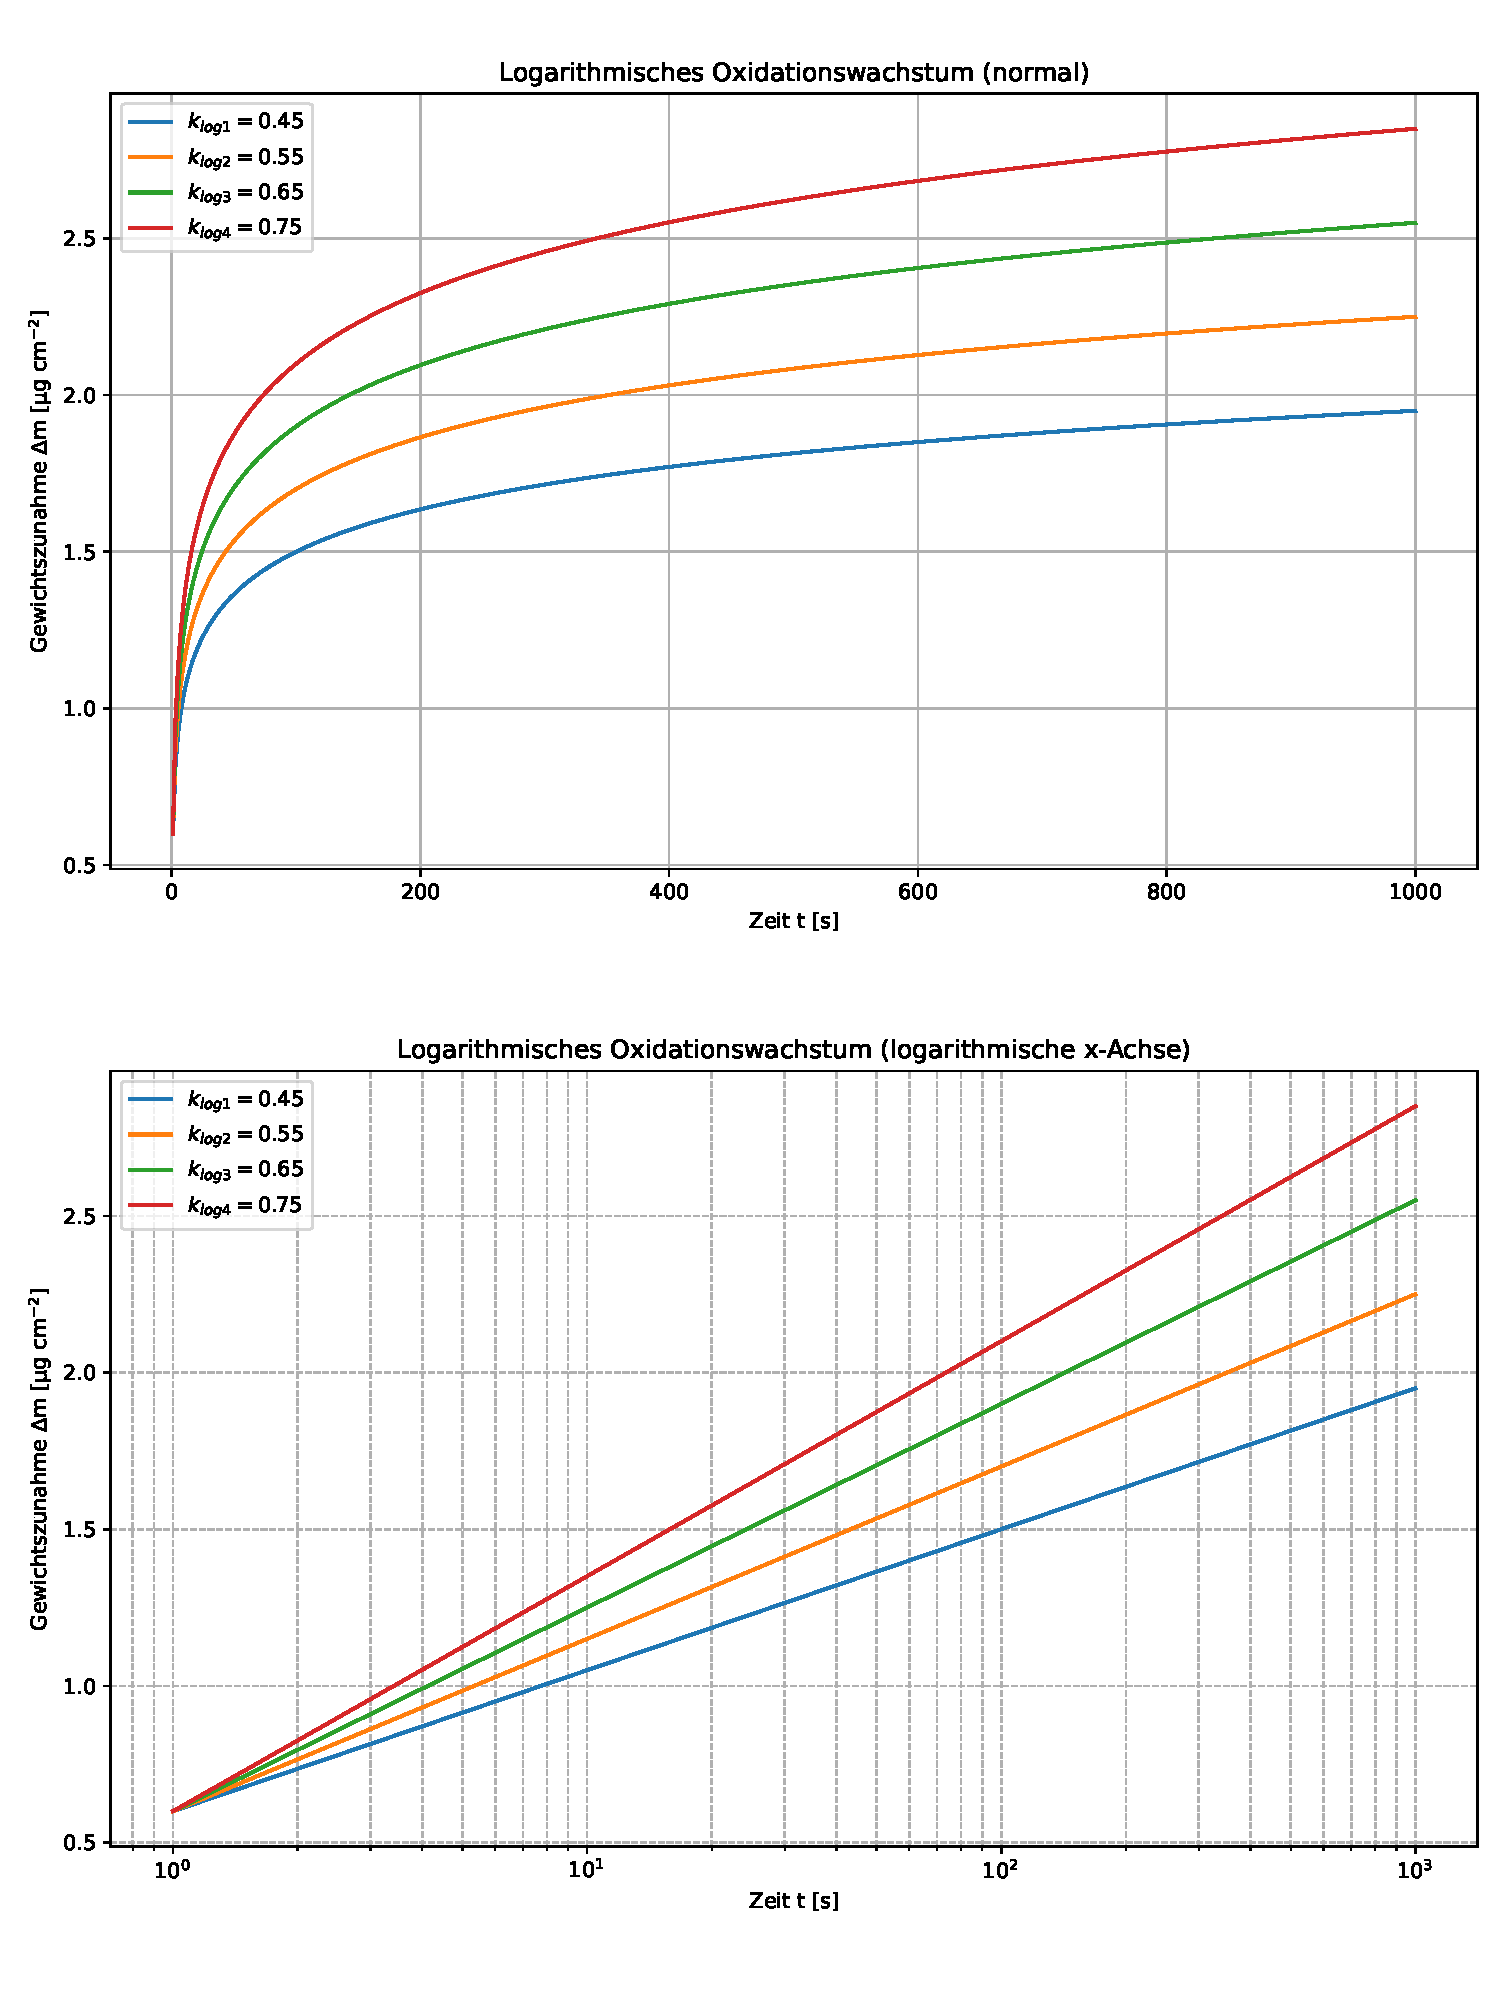
\includegraphics[width=\textwidth, page=1]{img/21/Plots_oxi.pdf}
    \caption{Entstandene Graphen aus der Gleichung, die in der Studie gegeben ist, mit verschiedenen $k_log$ konstanten und "Start"oxidation von 0,6.}
    \label{fig:log_3}
\end{figure}
\twocolumn